\documentclass[conference]{IEEEtran}
\IEEEoverridecommandlockouts
% The preceding line is only needed to identify funding in the first footnote. If that is unneeded, please comment it out.
\usepackage{cite}
\usepackage{amsmath,amssymb,amsfonts}
\usepackage{algorithmic}
\usepackage{graphicx}
\usepackage{textcomp}
\usepackage{xcolor}
\usepackage{hyperref}
\usepackage{float}
\def\BibTeX{{\rm B\kern-.05em{\sc i\kern-.025em b}\kern-.08em
    T\kern-.1667em\lower.7ex\hbox{E}\kern-.125emX}}
\begin{document}

\title{Dokumentation der Softwarearchitektur des Projekts Twitter-Dash}

% Authoren	
\author{
    \IEEEauthorblockN{Hahn, Bastian}
    \IEEEauthorblockA{
        \textit{b.hahn@oth-aw.de}\\
    }
    \and

    \IEEEauthorblockN{Kleber, Martin}
    \IEEEauthorblockA{
        \textit{m.kleber2@oth-aw.de}\\
    }
    \and

    \IEEEauthorblockN{Klier, Andreas}
    \IEEEauthorblockA{
        \textit{a.klier@oth-aw.de}\\
    }
    \and

    \IEEEauthorblockN{Kreussel, Lukas}
    \IEEEauthorblockA{
        \textit{l.kreussel@oth-aw.de}\\
    }
    \and

    \IEEEauthorblockN{Paris, Felix}
    \IEEEauthorblockA{
        \textit{f.paris1@oth-aw.de}\\
    }
    \and

    \IEEEauthorblockN{Ziegler, Andreas}
    \IEEEauthorblockA{
        \textit{a.ziegler1@oth-aw.de}\\
    }
}

\maketitle

\begin{abstract}
    In diesem technischem Report wird die Softwarearchitektur des Projekts
    Twitter-Dash vorgestellt. Das Projekt wurde im Rahmen der Vorlesung
    Big Data and Cloud Computing (bdcc) implementiert. Ziel der Implementierung ist es,
    ein Dashboard zu erstellen, dass aktuelle und historische Informationen zu Twitter Trends
    anzeigen und analysieren kann.
\end{abstract}

\begin{IEEEkeywords}
    Twitter, Big Data, Database, Web UI, Data Analysis
\end{IEEEkeywords}

\section{Introduction}
Bei der Applikation Twitter-Dash werden von der Twitter API alle 15 Min die aktuellen Trends
abgegriffen und in einer lokalen Datenbank gespeichert. Die Kommunikation zwischen den
einzelnen Services ist über eine gRPC Schnittstelle realisiert.
Die Interaktion des Anwenders mit der Applikation erfolgt dabei über eine Web-UI basierend auf dem
React Web-Framework.

\section{Architektur Allgemein}

Als Architektur wird ein Ansatz verfolgt, der sich stark an Microservices orientiert.
Dadurch wird eine abgeschlossene Logik von Front- und Backendkomponenten erreicht, die jeweils
von einem Subteam entwickelt wird. Diese gekapselten Einheiten können jeweils als isolierte Applikation der Containervisualisierung Docker betrieben werden.
Durch eine zentrale Konfigurationsdatei des Containers können diese zwischen den Teammitgliedern
ausgetauscht und ausgeführt werden. Damit wird eine hohe Portabilität gewährleistet.
Die Kommunikation der Teilsysteme wird durch eine sprachunabhängige gRPC-Schnittstelle angeboten.
Dadurch wird es möglich einzelne Komponenten des Gesamtsystems auszutauschen,
ohne größere Veränderungen an den anderen Microservices vornehmen zu müssen \cite{microservices}.

\begin{figure}
    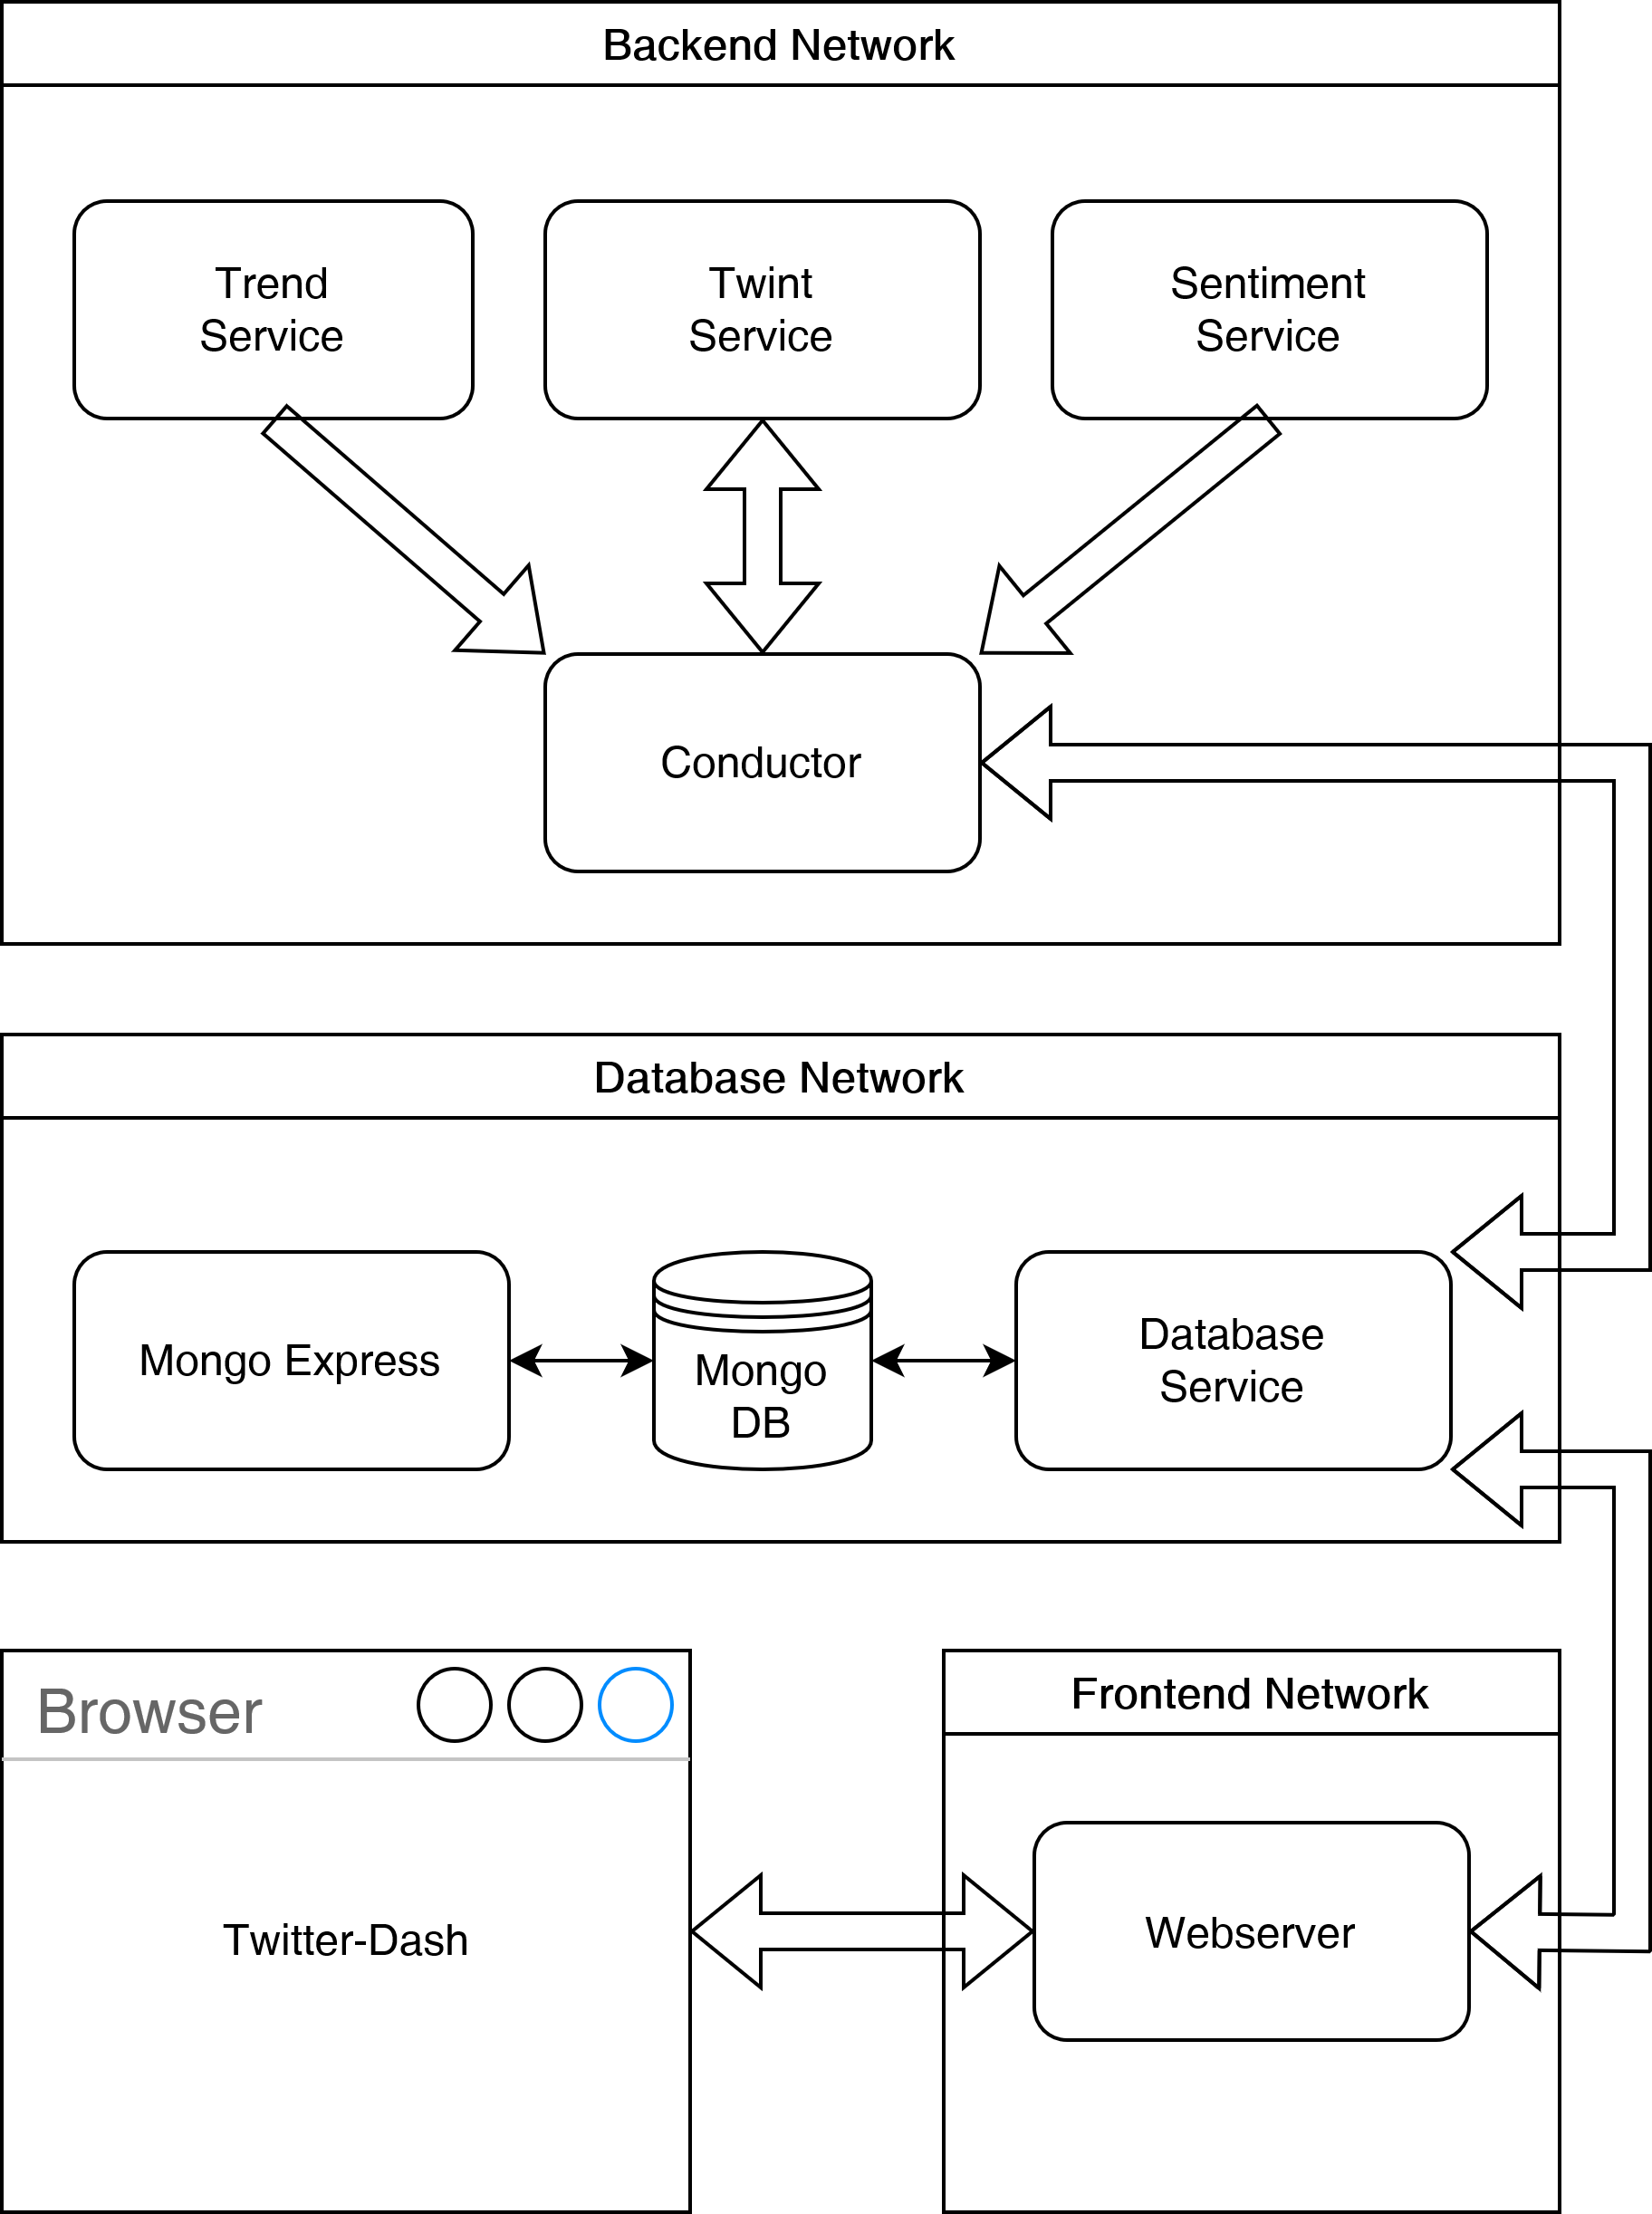
\includegraphics[width=0.5\textwidth]{Architecture.png}
    \caption{Übersicht Gesamtsystem}
\end{figure}


\section{Kommunikation}
Um Konflikten zwischen den Schnittstellen-Definitionen der einzelnen Dienste zu vermeiden,
wurden alle gRPC Schnittstellen in einem globalem Ordner definiert und vor  dem ausführen der Container über ein Script in die jeweiligen Source-Verzeichnisse der Dienste kopiert, bzw. wenn nötig mit dem gRPC-Tool kompiliert.
Dadurch werden Schnittstellen Änderungen gleichzeitig für alle Dienste vorgenommen.

%TODO Frontend


\section{Datenakquise}
Um Daten für das Dashboard zu erhalten, werden zwei unterschiedliche Vorgehensweisen verwendet.
Der verbreiteste Ansatz ist die Abfrage über die offizielle Twitter API \cite{twitterapi}.
Über diese werden die aktuellen Hashtags periodisch abgerufen.
Außerdem wurde Twint, ein fortgeschrittenes Scraping-Tool verwendet.
Dieses Tool liefert vollständige Tweets, inklusive zugehöriger Meta-Daten,
ohne direkten Zugriff auf die Twitter API zu benötigen \cite{twint}.

\subsection*{Trend-Service}
Für den Zugriff auf die Twitter-API wurde die Python-Bibliothek Tweepy \cite{tweepy} verwendet.
Diese Bibliothek bietet einen Client zur Verbindung zur Twitter-API.
Über diesen Client werden alle 15 Minuten die aktuellen Trends pro Land abgefragt und nach Hashtags gefiltert.
Diese werden über den Conductor zur Speicherung an die Datenbank gesendet.

Der Trend-Service bietet folgende Funktionen:
\begin{itemize}

    \item getAvailableTrends:\newline Liefert alle Länder zurück, für die die Twitter API aktuell Trends zur Verfügung stellt.
    \item getTrending:\newline Liefert die aktuellen Hashtags in einer Liste zurück. Die Listenelemente umfassen:
          \begin{itemize}
              \item Hashtag
              \item Platzierung nach Aktualität im Land
              \item Anzahl der Tweets zu diesem Hashtag
              \item Zeitstempel der Abfrage
              \item Land
          \end{itemize}
    \item getTweetCount:\newline Liefert die Anzahl der Tweets in einem vorgegebenen Zeitraum zu einem Hashtag zurück.

\end{itemize}

\subsection*{Twint-Service}
Da die Nutzung der Twitter-API eingeschränkt ist, wurde Twint verwendet, um viele Tweets zu laden.
Der Twint-Service wird nur auf Anfrage des Conductors ausgeführt.
Dieser gibt einen Hashtag, einen Start- und Endzeitpunktsangabe und eine Sprache vor.
Zu dieser Anfrage werden Tweets mit Twint gesammelt und nach Bereinigung von unwichtigen Metadaten zurück an den Conductor gegeben.

Die zurückgegebenen Elemente enthalten die folgenden Informationen:
\begin{itemize}
    \item Tweet-ID
    \item Conversation-ID
    \item Zeitstempel
    \item Textinhalt des Tweets
    \item Anzahl der Likes
    \item Anzahl der Retweets
    \item Hashtags in dem Tweet
    \item Sprache
\end{itemize}

\section{Datenverarbeitung}
Aus den gesammelten Daten können weitergehende Informationen extrahiert werden.
Hier wurde ein Service implementiert, der das Sentiment eines Tweets analysiert.

\subsection*{Sentiment-Analyse}
Bei der Sentimentanalyse werden die in einem Text ausgedrückten Meinungen mithilfe von NLP analysiert,
um festzustellen, wie die Einstellung des Verfassers zu einem bestimmten Thema ist.
Zur Analyse der Stimmungen wurden zwei verschiedene Modelle eingebunden,
ein bereits vortrainiertes neuronales Sprachmodell (BERT \cite{bert})
und ein ein stochastisches Modell (TextBlob \cite{textblob}).
Aufgrund des hohen Ressourcenverbrauchs des Tranformermodells (BERT) wurde das TextBlob-Modell für die Ausführung gewählt.

Die Ausführung der Sentiment-Analyse erfolgt über einen Service, der auf Anfrage des Conductors basiert.
Bei dieser Anfrage wird ein Text übergeben, der analysiert werden soll,
sowie eine Sprache, die zur Wahl des richtigen TextBlob-Modells benötigt wird.
Bevor der Text analysiert werden kann muss er bereinigt werden.
Dabei werden zum Beispiel unerwünschte Zeichen entfernt und die Zeichenkette in Kleinbuchstaben umgewandelt.
Als Ausgabe liefert der Service eine Zahlenwert zwischen -1 und 1.
Dabei wird der Wert -1 für negative und 1 für positive Stimmungen angenommen.


\section{Workflow}
Um die Zusammenarbeit zwischen den verschiedenen Datenakquise Diensten zu ermöglichen wurde ein Conductor-Service erstellt.
Der Dienst wurde in .Net 6 mit Hilfe der ELSA \cite{elsa} Open Source Workflow Library entwickelt.
Der Conductor Dienst enthält Client Implementierung für alle benötigen Dienste.
Für die Datenakquise wurden ein standard Workflow implementiert welcher die benötigen Daten von den anderen Diensten abruft und für weitere Verarbeitungsschritte aufbereitet.
Dieser Workflow wird durch das Erhalten von Trends des Trend-Services initialisiert und gestartet.
Über die ELSA-Bibliothek wird ein Web-Interface bereitgestellt, welches den aktuellen Status eines laufenden Workflows visualisiert, sowie Informationen und Ergebnisse von bereits ausgeführten Durchläufen enthält.

\begin{figure}[h]
    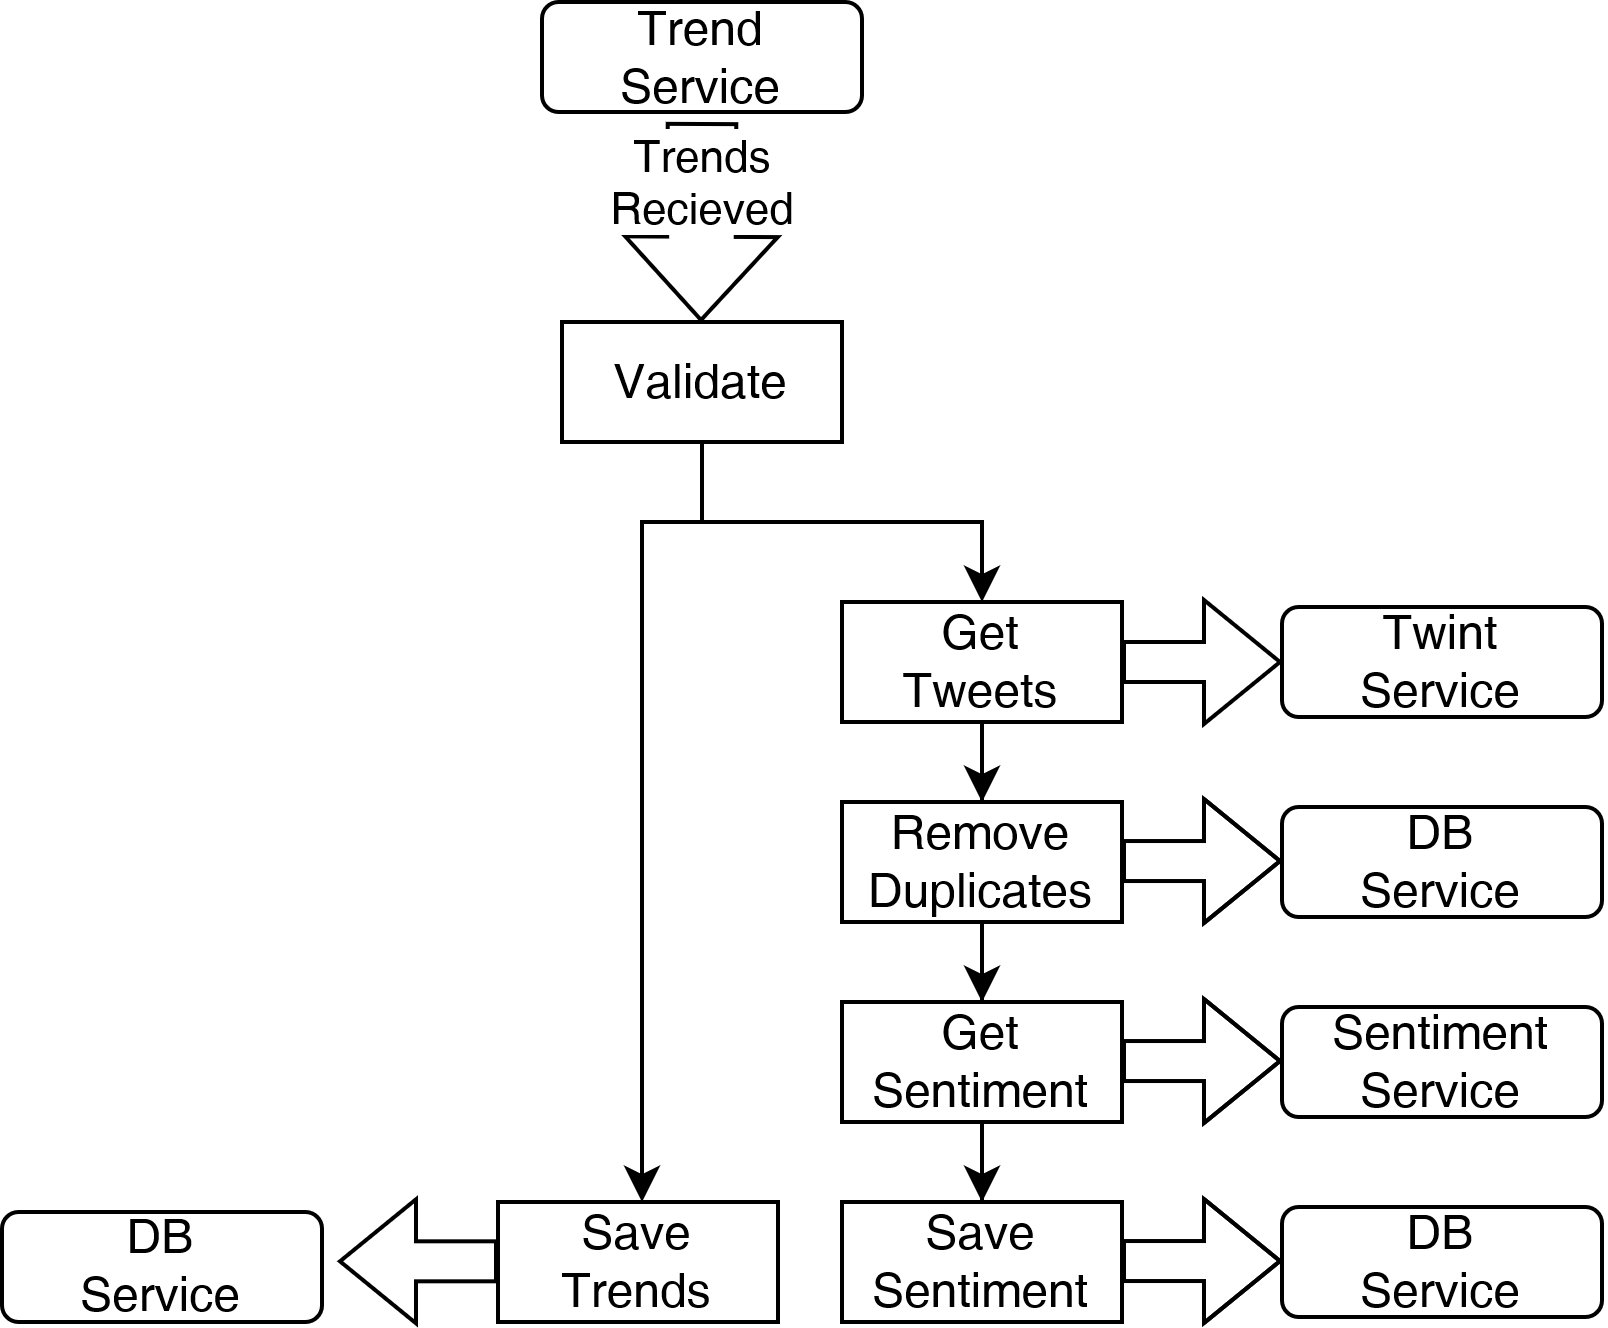
\includegraphics[width=0.5\textwidth]{Workflow.png}
    \caption{Standard Workflow}
\end{figure}


\section{Datenbank}
Alle Datenbankanfragen werden durch einen database service abstrahiert, der die Funktionen als gRPC
Schnittstelle anbietet. Dabei laufen die Datenbank und der database service in jeweils einem eigenen Container.
Durch die gRPC Schnittstelle können die Daten typsicher und Platform- sowie Programmiersprachen-unabhängig
an den database service übergeben und von diesem zurückgeliefert werden.
\\
Vom database service werden folgende Funktionen angeboten:
\\
Zum Speichern in die Datenbank:
\\
\smallskip
\textbf{Trends speichern (StoreTrends)}
\begin{itemize}
    \item Beschreibung: Speichert Trends in die Datenbank
    \item Parameter:
          \begin{itemize}
              \item Zeitstempel
              \item Liste von Trends mit folgenden Attributen:
                    \begin{itemize}
                        \item trendtype
                        \item name
                        \item country
                        \item placement
                        \item tweetVolume24
                    \end{itemize}
          \end{itemize}
    \item Rückgabe: Keine
\end{itemize}

\smallskip
\textbf{Sentiment speichern (StoreSentiment)}
\begin{itemize}
    \item Beschreibung: Speichert Sentiment in die Datenbank
    \item Parameter:
          \begin{itemize}
              \item Liste von Sentiments mit folgenden Attributen:
                    \begin{itemize}
                        \item tweet
                        \item Sentiment
                        \item topic
                    \end{itemize}
          \end{itemize}
    \item Rückgabe: Keine
\end{itemize}

zum Laden aus der Datenbank:
\\
\smallskip
\textbf{aktuelle Trends abrufen (GetCurrentTrends)}
\begin{itemize}
    \item Beschreibung: Lädt aktuelle Trends aus der Datenbank
    \item Parameter:
          \begin{itemize}
              \item country
              \item limit
          \end{itemize}
    \item Rückgabe:
          \begin{itemize}
              \item Zeitstempel
              \item Liste von Trends mit folgenden Attributen:
                    \begin{itemize}
                        \item trendtype
                        \item name
                        \item country
                        \item placement
                        \item tweetVolume24
                    \end{itemize}
          \end{itemize}
\end{itemize}

\smallskip
\textbf{vergangene Trends abrufen (GetRecentTrends)}
\begin{itemize}
    \item Beschreibung: Lädt vergangene Trends aus der Datenbank
    \item Parameter:
          \begin{itemize}
              \item hastag
              \item country
              \item startdate (optional)
              \item enddate (optional)
          \end{itemize}
    \item Rückgabe:
          \begin{itemize}
              \item Liste an Trends mit folgenden Attributen:
                    \begin{itemize}
                        \item Zeitstempel
                        \item Liste von Trends mit folgenden Attributen:
                              \begin{itemize}
                                  \item trendtype
                                  \item name
                                  \item country
                                  \item placement
                                  \item tweetVolume24
                              \end{itemize}
                    \end{itemize}
          \end{itemize}
\end{itemize}

\smallskip
\textbf{Vorhandene Länder abrufen (GetAvailableCountries)}
\begin{itemize}
    \item Beschreibung: Lädt vorhandene Länder aus der Datenbank
    \item Parameter: Keine
    \item Rückgabe: Liste mit allen Ländern, die in der Datenbak vorhanden sind
\end{itemize}

\smallskip
\textbf{Trends speichern (GetAvailableSentimentTrends)}
\begin{itemize}
    \item Beschreibung: Lädt vorhandene Trends aus der Datenbank
    \item Parameter:
          \begin{itemize}
              \item query
              \item limit
              \item country
          \end{itemize}
    \item Rückgabe: Liste an vorhandenen Sentiments
\end{itemize}

\smallskip
\textbf{aktuelle Sentiment abrufen (GetCurrentSentiment)}
\begin{itemize}
    \item Beschreibung: Lädt aktuellen Sentiment aus der Datenbank
    \item Parameter:
          \begin{itemize}
              \item Trendname
              \item Country
          \end{itemize}
    \item Rückgabe: Sentiment
\end{itemize}

\smallskip
\textbf{vergangene Sentiment abrufen (GetRecentSentiment)}
\begin{itemize}
    \item Beschreibung: Lädt vergangene Sentiment aus der Datenbank
    \item Parameter:
          \begin{itemize}
              \item Trendname
              \item Country
              \item startdate (optional)
              \item enddate (optional)
          \end{itemize}
    \item Rückgabe: Liste an Sentiments
\end{itemize}

\smallskip
\textbf{DB auf Tweet prüfen (GetUniqueTweets)}
\begin{itemize}
    \item Beschreibung: Gibt zurück, welche Tweets noch nicht in der Datenbank sind
    \item Parameter: Liste an Tweet IDs
    \item Rückgabe: Liste an Tweet IDs
\end{itemize}


\smallskip

Vom Backenend erzeugte Daten werden in einer MongoDB Datenbank gespeichert.
Dabei werden Trends zu bestimmten Zeitpunkten gespeichert. Diese enthalten Trendtype, Trendname, Placement, Country, TweetVolume24. Für Sentiments werden die Tweets, die zu einem Trend gehören, und das jeweilige Topic gespeichert.
\\
\\
Um die Funktionalität zu gewährleisten wurden Unit Tests entworfen. Dadurch kann die interne Integrität, sowie die Anbindung an externe Systeme,
sichergestellt werden. Die Tests wurden dabei mit dem Arrange-Act-Assert-Pattern entworfen. Dieses soll eine
übersichtliche Struktur und Einheitlichkeit garantieren.



\section{Frontend}
%TODO

\section{Testing}
Um die Funktionalität des Backends zu garantieren wurden alle Backend-Dienste mit einem zur verwendeten Programmiersprache passenden Unit-Test Framework getestet.
Die Code-Converage liegt dabei bei jeden Dienst über 90\%. 
%TODO

\begin{thebibliography}{0}
    \bibitem{microservices}Microservice-Frontend-Architekturen [Online] \url{https://www.sigs-datacom.de/uploads/tx_dmjournals/attermeyer_OTS_Microservices_Docker_16.pdf} (visited on Jun. 21, 2022)
    \bibitem{twitterapi}Twitter API [Online] \url{https://developer.twitter.com/en/docs/twitter-api} (visited on Jun. 23, 2022)
    \bibitem{twint}TWINT - Twitter Intelligence Tool [Online] \url{https://github.com/twintproject/twint} (visited on Jun. 23, 2022)
    \bibitem{tweepy}Tweepy: Twitter for Python! (2020) [Online] \url{https://github.com/tweepy/tweepy} (visited on Jun. 23, 2022)
    \bibitem{bert}bert-base-multilingual-uncased-sentiment [Online] \url{https://huggingface.co/nlptown/bert-base-multilingual-uncased-sentiment} (visited on Jun. 23, 2022)
    \bibitem{textblob}TextBlob: Simplified Text Processing [Online] \url{https://textblob.readthedocs.io/en/dev/} (visited on Jun. 23, 2022)
    \bibitem{elsa}ELSA - An open source .NET Standard workflow library [Online] \url{https://elsa-workflows.github.io/elsa-core/} (visited on Jun. 25, 2022)
\end{thebibliography}

\end{document}
